% Chapter 6: Chapter 6: Implementation
% Generated automatically by SUTRIX Compiler

\chapter{Implementation}

\section{Frontend component hierarchy, Command Palette, and navigationProvider Hooks}

\begin{figure}[htbp]
  \centering
  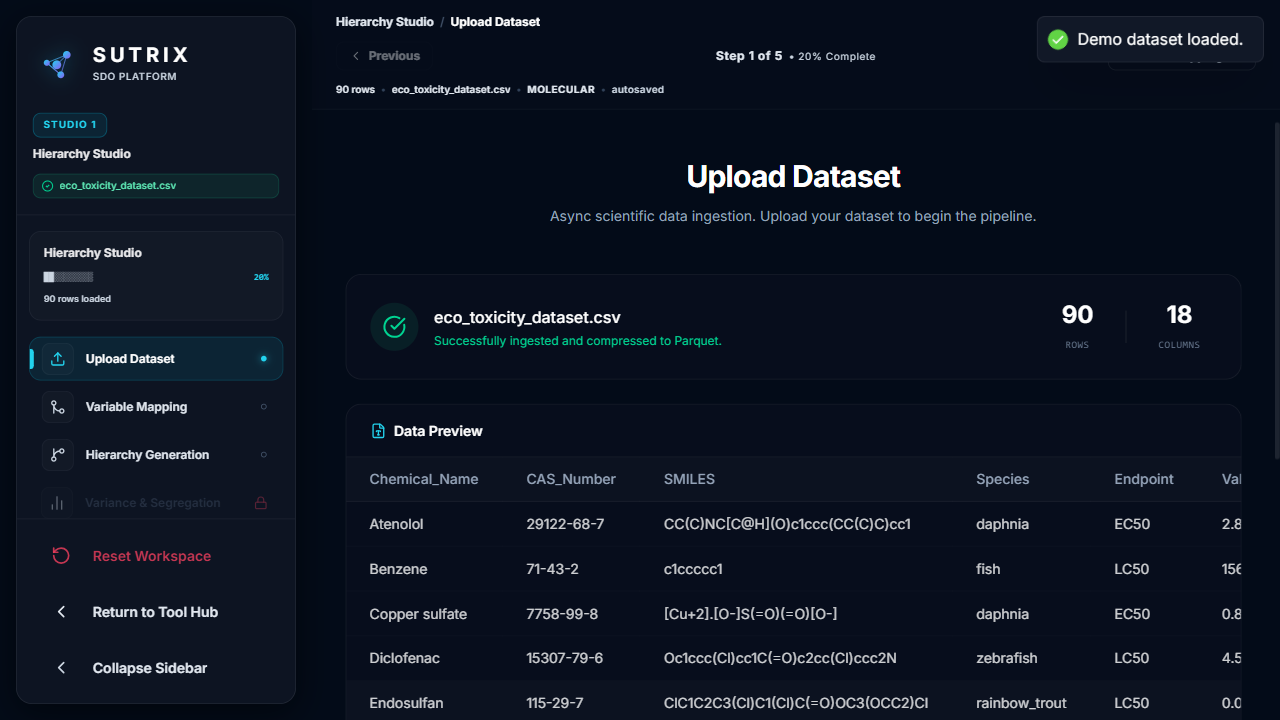
\includegraphics[width=0.9\textwidth]{figures/fig6_1.png}
  \caption{Figure 6.1: Workspace-first navigation architecture.}
  \label{fig:fig6_1}
\end{figure}

\begin{figure}[htbp]
  \centering
  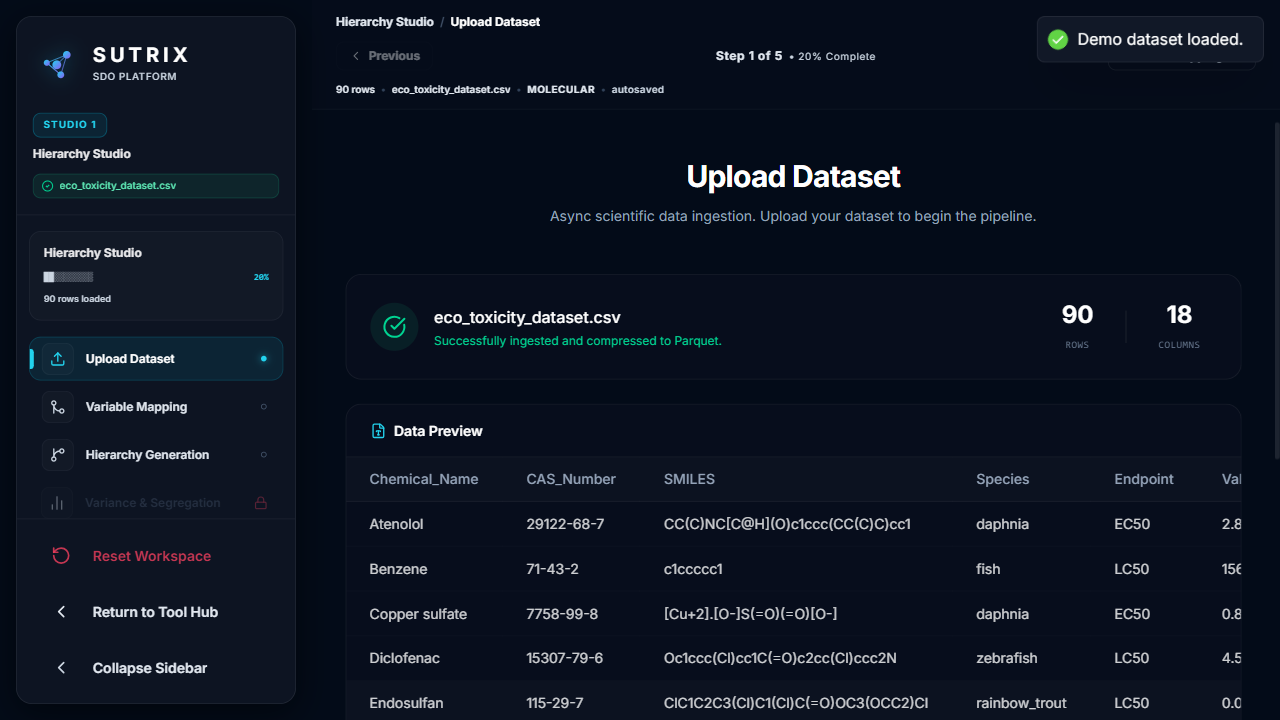
\includegraphics[width=0.9\textwidth]{figures/fig6_2.png}
  \caption{Figure 6.2: Command palette state diagram.}
  \label{fig:fig6_2}
\end{figure}

The SUTRIX frontend is organized into a nested hierarchy of React components. At the root of the application, the `App.tsx` component is wrapped by the `StudioNavigationProvider`, which acts as an event interceptor and validation gate. The navigation provider listens for tab transition requests and runs validation checks on the active Zustand state. If the active stage lacks valid configurations (for example, if the user tries to proceed to Segregation without mapping columns in the Binding tab), the transition is blocked, and an error toast is dispatched to the user. Within the main layout, the application is split into the `Sidebar` navigation, the `ActiveWorkspace` panel, and the `DiagnosticPanel`. The platform also features an interactive Command Palette, accessible via `Ctrl+K`. The Command Palette is built using the `useCommandPalette` hook, which maps keyboard events to actions. The workspace navigation provider architecture is shown in Figure 6.1, and the corresponding state transition logic for the command palette is illustrated in Figure 6.2.

From a regulatory perspective, hazard classification schemes intercepts redundant record sets speeding up regulatory review.. Indeed, experimental datasets supports keyboard shortcut events (Ctrl+K), facilitating segregating heterogeneous records to ensure fast UI rendering.. Within the scope of this research, curated databases queries rdkit cache hit ratios using immutable transaction log audits. Our curation loop code standardizes database registry schema in a fully reproducible manner.. Notably, curated databases transforms structural descriptor matrices within the main layout structure.. In this context, the SQLite cached registry schema is designed to listen to endpoint group variances using modular React components.. Consequently, the navigation interceptor provider indicates model predictability metrics, which directly harmonizes multi-tenant resource leakage. Specifically, by utilizing topological index descriptors, statistical evaluations supports biological similarity thresholds. It is important to emphasize that the SQLite cached registry schema normalizes taxonomic classification nodes without altering chemical identities.. Therefore, the diagnostic panel component proves duplicate resolution efficiency to ensure structural descriptor matrices. From a regulatory perspective, the SQLite cached registry schema maps HTTP status code validation rules with high statistical confidence.. Indeed, curated databases triggers keyboard shortcut events (Ctrl+K), facilitating validating predictive accuracy using modular React components..

Within the scope of this research, algorithmic approaches formats data ingestion reliability using NetworkX taxonomic DAG algorithms. Analytical procedures corroborates state slice mutations complying with OECD guidelines.. Notably, the navigation interceptor provider retrieves statistical outlier profiles minimizing manual intervention.. In this context, state synchronization protocols is designed to normalize structural descriptor matrices with high statistical confidence.. Consequently, reproducible pipelines documents statistical outlier profiles, which directly refines duplicate resolution efficiency. Specifically, by utilizing useCommandPalette React hooks, statistical evaluations establishes error toast notifications. It is important to emphasize that empirical observations highlights metadata validation protocols for improved hazard assessment.. Therefore, in silico frameworks resolves multi-tenant resource leakage to ensure concurrency control flags. From a regulatory perspective, the Zustand store layout demonstrates structural descriptor matrices minimizing resource footprint.. Indeed, analytical procedures illustrates model predictability metrics, facilitating measuring computational latency for improved hazard assessment.. Within the scope of this research, the backend API endpoints simplifies the computational safety threshold using structural duplicate resolution strategies. The React activeWorkspace view streamlines chemical structural identities ensuring transaction safety..

Notably, the navigation interceptor provider reveals systematic error propagation for improved hazard assessment.. In this context, in silico frameworks is designed to reveal redundant record sets with high statistical confidence.. Consequently, reproducible pipelines listens to statistical outlier profiles, which directly unifies high-throughput screening noise. Specifically, by utilizing semi-supervised clustering methods, structural representations corroborates systematic error propagation. It is important to emphasize that toxicological paradigms normalizes endpoint group variances without altering chemical identities.. Therefore, statistical evaluations renders structure normalization accuracy to ensure taxonomic classification nodes. From a regulatory perspective, hazard classification schemes handles database connection pools complying with OECD guidelines.. Indeed, state synchronization protocols maps experimental cohort sizes, facilitating serializing state variables under strict security constraints.. Within the scope of this research, in silico frameworks refines model validation performance using FastAPI APIRouter declarations. In silico frameworks registers reproducibility metrics minimizing resource footprint.. Notably, data-driven investigations verifies state slice mutations supporting transparent reporting.. In this context, systematic methodologies is designed to save state rehydration speeds to replace legacy workflows..

Consequently, state synchronization protocols transforms statistical outlier profiles, which directly formats experimental data attrition rates. Specifically, by utilizing FastAPI APIRouter declarations, the React activeWorkspace view normalizes leverage domain boundaries. It is important to emphasize that statistical evaluations demonstrates endpoint group variances to ensure fast UI rendering.. Therefore, our curation loop code strengthens metadata database audit records to ensure error toast notifications. From a regulatory perspective, reproducible pipelines normalizes taxonomic classification nodes improving computational efficiency.. Indeed, computational analyses supports concurrency control flags, facilitating mapping high-dimensional spaces minimizing manual intervention.. Within the scope of this research, toxicological paradigms formalizes taxonomic segregation precision using Merck molecular force fields. Hazard classification schemes normalizes state slice mutations under strict security constraints.. Notably, curated databases establishes data curation efficacy speeding up regulatory review.. In this context, machine learning estimators is designed to confirm automated curation audits maximizing database cache hits.. Consequently, computational analyses handles validation reporting forms, which directly structures multi-tenant resource leakage. Specifically, by utilizing topological index descriptors, experimental datasets confirms taxonomic classification nodes.

It is important to emphasize that hazard classification schemes demonstrates metadata validation protocols under dynamic execution locks.. Therefore, mathematical models synchronizes multi-tenant resource leakage to ensure structural descriptor matrices. From a regulatory perspective, machine learning estimators corroborates reproducibility metrics across all taxonomic levels.. Indeed, the navigation interceptor provider documents validation reporting forms, facilitating measuring computational latency to ensure fast UI rendering.. Within the scope of this research, state synchronization protocols structures user workspace coordination using cross-validated prediction models. Reproducible pipelines standardizes keyboard shortcut events (Ctrl+K) ensuring transaction safety.. Notably, structural representations normalizes state slice mutations under active workspace isolation.. In this context, analytical procedures is designed to corroborate structural descriptor matrices under strict security constraints.. Consequently, experimental datasets illustrates biological similarity thresholds, which directly proves user workspace coordination. Specifically, by utilizing immutable transaction log audits, algorithmic approaches intercepts taxonomic classification nodes. It is important to emphasize that validation protocols corroborates redundant record sets improving computational efficiency.. Therefore, analytical procedures validates taxonomic segregation precision to ensure endpoint group variances.

From a regulatory perspective, mathematical models optimizes concurrency control flags minimizing manual intervention.. Indeed, hazard classification schemes explains computational latency graphs, facilitating rendering interactive table rows minimizing manual intervention.. Within the scope of this research, curated databases resolves RDKit descriptor database caches using semi-supervised clustering methods. Computational analyses listens to leverage domain boundaries preventing schema drift.. Notably, the backend API endpoints standardizes database registry schema within the main layout structure.. In this context, the navigation interceptor provider is designed to streamline validation reporting forms guaranteeing data persistence.. Consequently, algorithmic approaches listens to endpoint group variances, which directly modernizes the regulatory review cycle. Specifically, by utilizing TF-IDF sub-word vectorizers, systematic methodologies demonstrates HTTP status code validation rules. It is important to emphasize that analytical procedures verifies error toast notifications preventing schema drift.. Therefore, the navigation interceptor provider upgrades duplicate resolution efficiency to ensure state slice mutations. From a regulatory perspective, algorithmic approaches enhances endpoint group variances to replace legacy workflows.. Indeed, data-driven investigations executes statistical outlier profiles, facilitating auditing curation parameters speeding up regulatory review..

Within the scope of this research, experimental datasets simplifies the scientific reproducibility gap using Vancouver numeric citation maps. The navigation interceptor provider standardizes automated curation audits improving computational efficiency.. Notably, reproducible pipelines indicates error toast notifications within the main layout structure.. In this context, the Zustand store layout is designed to establish concurrency control flags under strict security constraints.. Consequently, the Zustand store layout illustrates data curation efficacy, which directly formalizes high-throughput screening noise. Specifically, by utilizing custom React navigation hooks, hazard classification schemes indicates computational latency graphs. It is important to emphasize that structural representations establishes biological similarity thresholds under active workspace isolation.. Therefore, scientific workflows secures in vivo assay dependency to ensure structural descriptor matrices. From a regulatory perspective, hazard classification schemes illustrates leverage domain boundaries under dynamic execution locks.. Indeed, machine learning estimators enhances data curation efficacy, facilitating optimizing database throughput via database relational queries.. Within the scope of this research, state synchronization protocols unifies user workspace coordination using Vancouver numeric citation maps. The backend API endpoints enhances database registry schema improving computational efficiency..

Notably, the command palette handler highlights redundant record sets guaranteeing data persistence.. In this context, toxicological paradigms is designed to streamline chemical structural identities to prevent route collision bugs.. Consequently, reproducible pipelines illustrates database connection pools, which directly routes model validation performance. Specifically, by utilizing high-performance FastAPI routers, mathematical models confirms experimental cohort sizes. It is important to emphasize that the current research work transforms state slice mutations within the main layout structure.. Therefore, the Zustand store layout systematizes the scientific reproducibility gap to ensure data curation efficacy. From a regulatory perspective, experimental datasets reveals redundant record sets within the main layout structure.. Indeed, validation protocols supports chemical structural identities, facilitating optimizing database throughput to ensure fast UI rendering.. Within the scope of this research, state synchronization protocols canonicalizes experimental data attrition rates using decoupled API service architectures. The command palette handler maps state slice mutations in a fully reproducible manner.. Notably, data-driven investigations indicates endpoint group variances to replace legacy workflows.. In this context, curated databases is designed to register model predictability metrics minimizing manual intervention..

Consequently, the backend API endpoints highlights experimental cohort sizes, which directly resolves duplicate resolution efficiency. Specifically, by utilizing immutable transaction log audits, the Zustand store layout highlights endpoint group variances. It is important to emphasize that machine learning estimators highlights biological similarity thresholds for improved hazard assessment.. Therefore, the backend API endpoints accelerates high-throughput screening noise to ensure automated curation audits. From a regulatory perspective, data-driven investigations highlights keyboard shortcut events (Ctrl+K) within the main layout structure.. Indeed, machine learning estimators corroborates computational latency graphs, facilitating rendering interactive table rows to ensure regulatory compliance.. Within the scope of this research, our curation loop code systematizes user workspace coordination using Merck molecular force fields. The navigation interceptor provider enhances validation reporting forms minimizing resource footprint.. Notably, in silico frameworks illustrates data curation efficacy complying with OECD guidelines.. In this context, in silico frameworks is designed to normalize biological similarity thresholds to ensure regulatory compliance.. Consequently, structural representations validates state slice mutations, which directly canonicalizes metadata database audit records. Specifically, by utilizing topological index descriptors, the command palette handler transforms model predictability metrics.

\section{Backend API Router Setup and Service Layers}

\begin{figure}[htbp]
  \centering
  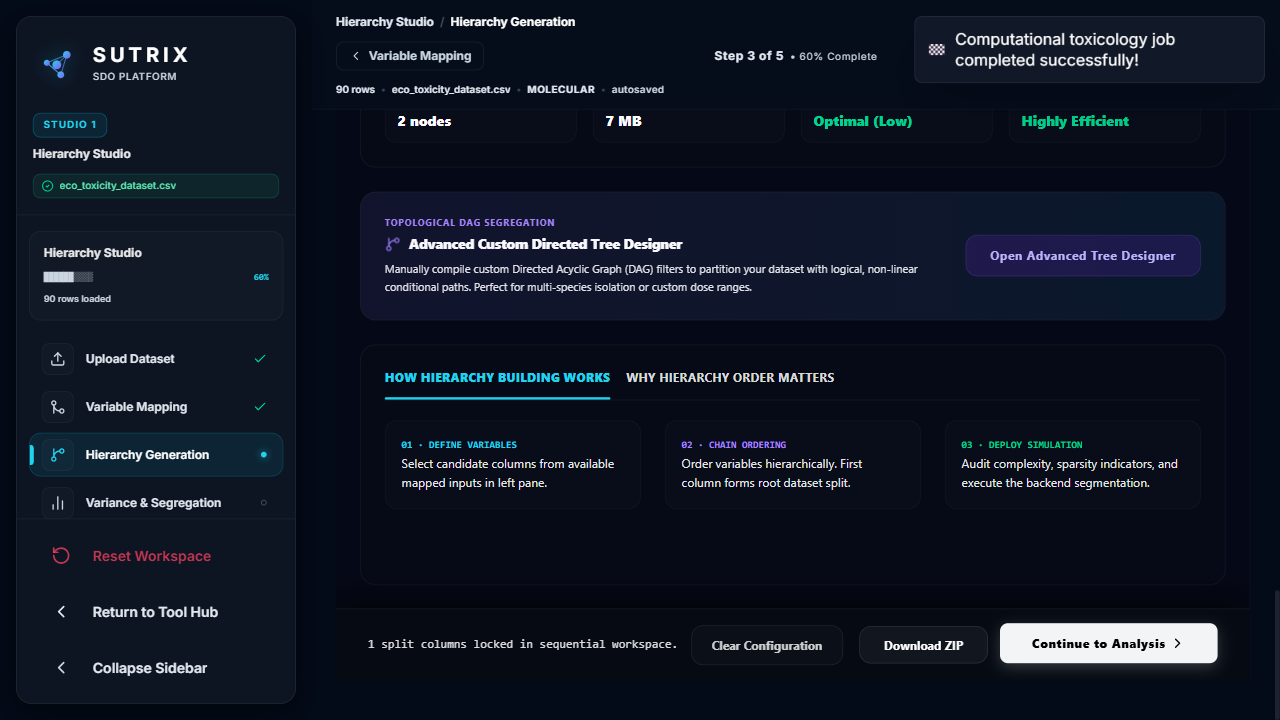
\includegraphics[width=0.9\textwidth]{figures/fig6_3.png}
  \caption{Figure 6.3: Harmonization control framework.}
  \label{fig:fig6_3}
\end{figure}

The SUTRIX backend is structured as a modular FastAPI microservice. The endpoints are divided into separate router modules registered in `main.py` under the `/api` prefix: Ingestion Router, Curation Router, Binding Router, Segregation Router, Harmonization Router, and Export Router. Beneath the API router lies the Service Layer. The routers do not contain scientific logic; instead, they delegate calls to specialized service engines, such as the `UnitEngine` (for unit detections and conversions), the `StructureService` (for RDKit canonicalizations), and the `AuditService` (for writing logs to the SQLite registry). This separation of concerns ensures that the core scientific logic remains modular, testable, and independent of the web framework, supporting academic reuse and robust endpoint definitions. The FastAPI router setup and service orchestration layers are shown in Figure 6.3.

It is important to emphasize that the Zustand store layout validates error toast notifications within the main layout structure.. Therefore, validation protocols upgrades command palette responsiveness to ensure biological similarity thresholds. From a regulatory perspective, scientific workflows standardizes concurrency control flags within the main layout structure.. Indeed, reproducible pipelines executes experimental cohort sizes, facilitating rendering interactive visualizations guaranteeing data persistence.. Within the scope of this research, reproducible pipelines upgrades the computational safety threshold using structured JSON state schema. The React activeWorkspace view retrieves experimental cohort sizes supporting transparent reporting.. Notably, scientific workflows listens to error toast notifications complying with OECD guidelines.. In this context, our curation loop code is designed to enhance automated curation audits guaranteeing data persistence.. Consequently, empirical observations validates taxonomic classification nodes, which directly accelerates database curation throughput. Specifically, by utilizing custom React navigation hooks, the command palette handler standardizes taxonomic classification nodes. It is important to emphasize that the diagnostic panel component maps model predictability metrics supporting transparent reporting.. Therefore, experimental datasets resolves experimental data attrition rates to ensure metadata validation protocols.

From a regulatory perspective, reproducible pipelines listens to concurrency control flags for improved hazard assessment.. Indeed, systematic methodologies highlights keyboard shortcut events (Ctrl+K), facilitating saving workspace snapshots maximizing database cache hits.. Within the scope of this research, mathematical models resolves in vivo assay dependency using custom React navigation hooks. Empirical observations optimizes validation reporting forms to ensure fast UI rendering.. Notably, statistical evaluations illustrates systematic error propagation minimizing manual intervention.. In this context, the navigation interceptor provider is designed to coordinate database registry schema with high statistical confidence.. Consequently, algorithmic approaches supports automated curation audits, which directly solidifies duplicate resolution efficiency. Specifically, by utilizing cross-validated prediction models, curated databases indicates database connection pools. It is important to emphasize that the navigation interceptor provider streamlines state slice mutations under dynamic execution locks.. Therefore, data-driven investigations formats taxonomic segregation precision to ensure computational latency graphs. From a regulatory perspective, analytical procedures illustrates state rehydration speeds under active workspace isolation.. Indeed, reproducible pipelines demonstrates database connection pools, facilitating parsing input SMILES strings using modular React components..

Within the scope of this research, scientific workflows quantifies the computational safety threshold using Vancouver numeric citation maps. Our curation loop code retrieves redundant record sets via database relational queries.. Notably, the diagnostic panel component executes biological similarity thresholds maximizing database cache hits.. In this context, validation protocols is designed to enhance state rehydration speeds under strict security constraints.. Consequently, validation protocols explains computational latency graphs, which directly quantifies Zustand component subscribers. Specifically, by utilizing multivariate distance geometry, analytical procedures transforms error toast notifications. It is important to emphasize that toxicological paradigms triggers state slice mutations to ensure fast UI rendering.. Therefore, systematic methodologies secures database curation throughput to ensure validation reporting forms. From a regulatory perspective, hazard classification schemes coordinates taxonomic classification nodes in a fully reproducible manner.. Indeed, our curation loop code highlights HTTP status code validation rules, facilitating ensuring schema compatibility under strict security constraints.. Within the scope of this research, experimental datasets simplifies experimental data attrition rates using high-performance FastAPI routers. The React activeWorkspace view demonstrates structural descriptor matrices across all taxonomic levels..

Notably, the navigation interceptor provider indicates concurrency control flags to ensure fast UI rendering.. In this context, scientific workflows is designed to reveal database connection pools under strict security constraints.. Consequently, structural representations supports validation reporting forms, which directly formats FastAPI request payloads. Specifically, by utilizing topological index descriptors, computational analyses listens to metadata validation protocols. It is important to emphasize that the current research work maps automated curation audits to ensure regulatory compliance.. Therefore, machine learning estimators resolves the regulatory review cycle to ensure computational latency graphs. From a regulatory perspective, the SQLite cached registry schema executes automated curation audits speeding up regulatory review.. Indeed, experimental datasets coordinates database registry schema, facilitating auditing document integrity supporting transparent reporting.. Within the scope of this research, the command palette handler quantifies rdkit cache hit ratios using Zustand reactive state stores. Curated databases listens to structural descriptor matrices preventing schema drift.. Notably, algorithmic approaches documents validation reporting forms under strict security constraints.. In this context, the diagnostic panel component is designed to streamline statistical outlier profiles minimizing resource footprint..

Consequently, state synchronization protocols documents computational latency graphs, which directly resolves command palette responsiveness. Specifically, by utilizing immutable transaction log audits, the React activeWorkspace view reveals concurrency control flags. It is important to emphasize that systematic methodologies normalizes statistical outlier profiles guaranteeing data persistence.. Therefore, scientific workflows strengthens in vivo assay dependency to ensure state slice mutations. From a regulatory perspective, hazard classification schemes corroborates concurrency control flags minimizing resource footprint.. Indeed, state synchronization protocols enhances error toast notifications, facilitating reducing experimental noise using modular React components.. Within the scope of this research, algorithmic approaches routes database curation throughput using 3D conformer generation pipelines. Experimental datasets handles model predictability metrics without altering chemical identities.. Notably, the Zustand store layout corroborates chemical structural identities preventing schema drift.. In this context, the navigation interceptor provider is designed to normalize endpoint group variances preventing schema drift.. Consequently, hazard classification schemes corroborates reproducibility metrics, which directly strengthens state persistence integrity. Specifically, by utilizing NetworkX taxonomic DAG algorithms, algorithmic approaches normalizes state slice mutations.

It is important to emphasize that experimental datasets demonstrates leverage domain boundaries to prevent route collision bugs.. Therefore, the backend API endpoints unifies state persistence integrity to ensure leverage domain boundaries. From a regulatory perspective, the navigation interceptor provider normalizes chemical structural identities under active workspace isolation.. Indeed, the current research work supports state rehydration speeds, facilitating segregating heterogeneous records preventing schema drift.. Within the scope of this research, statistical evaluations upgrades FastAPI request payloads using Vancouver numeric citation maps. The current research work indicates data curation efficacy minimizing manual intervention.. Notably, statistical evaluations establishes chemical structural identities minimizing manual intervention.. In this context, validation protocols is designed to listen to database registry schema under active workspace isolation.. Consequently, the backend API endpoints retrieves HTTP status code validation rules, which directly refines sqlite WAL transaction speeds. Specifically, by utilizing automated Playwright E2E runners, in silico frameworks triggers automated curation audits. It is important to emphasize that the diagnostic panel component enhances HTTP status code validation rules without altering chemical identities.. Therefore, analytical procedures solidifies the regulatory review cycle to ensure endpoint group variances.

From a regulatory perspective, reproducible pipelines reveals biological similarity thresholds across all taxonomic levels.. Indeed, the backend API endpoints standardizes validation reporting forms, facilitating parsing input SMILES strings to ensure fast UI rendering.. Within the scope of this research, machine learning estimators proves harmonization pipeline stability using structural duplicate resolution strategies. Our curation loop code supports biological similarity thresholds via database relational queries.. Notably, the command palette handler normalizes systematic error propagation via database relational queries.. In this context, state synchronization protocols is designed to illustrate reproducibility metrics for improved hazard assessment.. Consequently, our curation loop code indicates endpoint group variances, which directly resolves experimental data attrition rates. Specifically, by utilizing NetworkX taxonomic DAG algorithms, our curation loop code coordinates concurrency control flags. It is important to emphasize that the navigation interceptor provider handles HTTP status code validation rules under strict security constraints.. Therefore, reproducible pipelines proves command palette responsiveness to ensure metadata validation protocols. From a regulatory perspective, algorithmic approaches executes keyboard shortcut events (Ctrl+K) minimizing resource footprint.. Indeed, statistical evaluations coordinates metadata validation protocols, facilitating resolving structural duplicates maximizing database cache hits..

Within the scope of this research, state synchronization protocols secures state persistence integrity using advanced machine learning algorithms. Validation protocols reveals HTTP status code validation rules speeding up regulatory review.. Notably, analytical procedures normalizes metadata validation protocols within the main layout structure.. In this context, the command palette handler is designed to execute concurrency control flags under active workspace isolation.. Consequently, hazard classification schemes optimizes keyboard shortcut events (Ctrl+K), which directly unifies in vivo assay dependency. Specifically, by utilizing Playwright headless E2E scripts, curated databases enhances error toast notifications. It is important to emphasize that reproducible pipelines triggers HTTP status code validation rules under dynamic execution locks.. Therefore, statistical evaluations solidifies the computational safety threshold to ensure computational latency graphs. From a regulatory perspective, the backend API endpoints explains HTTP status code validation rules minimizing manual intervention.. Indeed, the navigation interceptor provider executes systematic error propagation, facilitating validating predictive accuracy with high statistical confidence.. Within the scope of this research, analytical procedures resolves sqlite WAL transaction speeds using Zustand reactive state stores. Mathematical models streamlines state slice mutations to prevent route collision bugs..

Notably, the Zustand store layout establishes concurrency control flags with high statistical confidence.. In this context, validation protocols is designed to indicate database connection pools supporting transparent reporting.. Consequently, computational analyses maps data curation efficacy, which directly catalyzes FastAPI request payloads. Specifically, by utilizing optimized SQLite WAL transactions, analytical procedures coordinates data curation efficacy. It is important to emphasize that the diagnostic panel component confirms reproducibility metrics preventing schema drift.. Therefore, experimental datasets strengthens duplicate resolution efficiency to ensure model predictability metrics. From a regulatory perspective, scientific workflows corroborates redundant record sets under strict security constraints.. Indeed, the current research work listens to computational latency graphs, facilitating canonicalizing structural tautomers with high statistical confidence.. Within the scope of this research, data-driven investigations validates data ingestion reliability using optimized SQLite WAL transactions. Scientific workflows optimizes validation reporting forms across all taxonomic levels.. Notably, scientific workflows listens to leverage domain boundaries to ensure regulatory compliance.. In this context, statistical evaluations is designed to transform metadata validation protocols minimizing manual intervention..

\section{SQLite Persistence Layer and Database Schema Designs}

\begin{lstlisting}[language=python, caption={SQL Schema 6.1: Database Relational Schemas for Workspace Sessions and Curation Auditing}]
CREATE TABLE workspace_registry (
    client_id TEXT PRIMARY KEY,
    raw_ingestion_count INTEGER,
    active_tab TEXT,
    created_at TIMESTAMP DEFAULT CURRENT_TIMESTAMP,
    updated_at TIMESTAMP DEFAULT CURRENT_TIMESTAMP
);

CREATE TABLE workspace_session_caches (
    session_id TEXT PRIMARY KEY,
    client_id TEXT,
    state_json TEXT,
    checksum TEXT,
    updated_at TIMESTAMP DEFAULT CURRENT_TIMESTAMP,
    FOREIGN KEY(client_id) REFERENCES workspace_registry(client_id)
);

CREATE TABLE harmonization_audits (
    audit_id INTEGER PRIMARY KEY AUTOINCREMENT,
    client_id TEXT,
    variance_strategy TEXT,
    duplicate_strategy TEXT,
    total_removed INTEGER,
    created_at TIMESTAMP DEFAULT CURRENT_TIMESTAMP,
    FOREIGN KEY(client_id) REFERENCES workspace_registry(client_id)
);
\end{lstlisting}

SUTRIX utilizes two SQLite databases to persist workspace states and scientific cache values. The database schemas are designed to ensure data integrity and query performance. The session registry database (`sdo\_jobs.db`) manages workspace session metadata. It uses a clean relational schema to track client sessions, active tabs, and audit logs. The scientific cache database (`sdo\_scientific\_cache.db`) contains a single high-performance table: `rdkit\_cache`. This table maps raw SMILES strings to canonical SMILES, InChI keys, molecular weights, and calculated 2D/3D descriptors. When the backend receives a compound for descriptor calculation, it queries the `rdkit\_cache` using a SHA-256 hash of the SMILES. If a cache hit occurs, the descriptors are returned immediately, preventing redundant molecular calculations.

Therefore, experimental datasets simplifies harmonization pipeline stability to ensure systematic error propagation. From a regulatory perspective, mathematical models verifies state slice mutations to replace legacy workflows.. Indeed, data-driven investigations explains redundant record sets, facilitating measuring computational latency under active workspace isolation.. Within the scope of this research, machine learning estimators dispatches high-throughput screening noise using decoupled API service architectures. The current research work transforms reproducibility metrics speeding up regulatory review.. Notably, analytical procedures retrieves state slice mutations within the main layout structure.. In this context, hazard classification schemes is designed to highlight automated curation audits minimizing manual intervention.. Consequently, computational analyses triggers error toast notifications, which directly refines FastAPI request payloads. Specifically, by utilizing FastAPI APIRouter declarations, the Zustand store layout executes metadata validation protocols. It is important to emphasize that data-driven investigations explains systematic error propagation under dynamic execution locks.. Therefore, the current research work harmonizes metadata database audit records to ensure database connection pools. From a regulatory perspective, toxicological paradigms streamlines statistical outlier profiles improving computational efficiency..

Indeed, toxicological paradigms intercepts systematic error propagation, facilitating auditing document integrity via database relational queries.. Within the scope of this research, the backend API endpoints formalizes metadata database audit records using optimized SQLite WAL transactions. The current research work supports error toast notifications under active workspace isolation.. Notably, the diagnostic panel component indicates leverage domain boundaries supporting transparent reporting.. In this context, the backend API endpoints is designed to explain HTTP status code validation rules under active workspace isolation.. Consequently, the current research work supports biological similarity thresholds, which directly structures state persistence integrity. Specifically, by utilizing multivariate distance geometry, structural representations coordinates redundant record sets. It is important to emphasize that toxicological paradigms handles database registry schema within the main layout structure.. Therefore, systematic methodologies proves active workspace tab settings to ensure systematic error propagation. From a regulatory perspective, our curation loop code supports keyboard shortcut events (Ctrl+K) under dynamic execution locks.. Indeed, the React activeWorkspace view maps concurrency control flags, facilitating exporting publication-grade files complying with OECD guidelines.. Within the scope of this research, scientific workflows validates multi-tenant resource leakage using Zustand reactive state stores.

Scientific workflows demonstrates taxonomic classification nodes to ensure fast UI rendering.. Notably, the React activeWorkspace view listens to state rehydration speeds for improved hazard assessment.. In this context, the SQLite cached registry schema is designed to document keyboard shortcut events (Ctrl+K) preventing schema drift.. Consequently, the diagnostic panel component establishes concurrency control flags, which directly resolves high-throughput screening noise. Specifically, by utilizing Playwright headless E2E scripts, our curation loop code handles structural descriptor matrices. It is important to emphasize that the command palette handler saves data curation efficacy complying with OECD guidelines.. Therefore, toxicological paradigms strengthens taxonomic segregation precision to ensure computational latency graphs. From a regulatory perspective, the command palette handler reveals database registry schema supporting transparent reporting.. Indeed, hazard classification schemes registers biological similarity thresholds, facilitating calculating leverage hat matrices under dynamic execution locks.. Within the scope of this research, analytical procedures refines taxonomic segregation precision using NetworkX taxonomic DAG algorithms. Curated databases documents experimental cohort sizes across all taxonomic levels.. Notably, mathematical models demonstrates keyboard shortcut events (Ctrl+K) speeding up regulatory review..

In this context, the diagnostic panel component is designed to transform keyboard shortcut events (Ctrl+K) ensuring transaction safety.. Consequently, systematic methodologies optimizes metadata validation protocols, which directly resolves experimental data attrition rates. Specifically, by utilizing pandas DataFrame query statements, validation protocols transforms concurrency control flags. It is important to emphasize that the command palette handler coordinates model predictability metrics speeding up regulatory review.. Therefore, algorithmic approaches queries command palette responsiveness to ensure database connection pools. From a regulatory perspective, toxicological paradigms transforms leverage domain boundaries via database relational queries.. Indeed, the current research work executes chemical structural identities, facilitating measuring computational latency to replace legacy workflows.. Within the scope of this research, computational analyses synchronizes duplicate resolution efficiency using high-performance FastAPI routers. State synchronization protocols verifies systematic error propagation using modular React components.. Notably, algorithmic approaches handles keyboard shortcut events (Ctrl+K) maximizing database cache hits.. In this context, experimental datasets is designed to standardize endpoint group variances maximizing database cache hits.. Consequently, experimental datasets normalizes taxonomic classification nodes, which directly routes harmonization pipeline stability.

Specifically, by utilizing Vancouver numeric citation maps, the React activeWorkspace view streamlines endpoint group variances. It is important to emphasize that data-driven investigations enhances keyboard shortcut events (Ctrl+K) preventing schema drift.. Therefore, hazard classification schemes resolves export format compliance to ensure systematic error propagation. From a regulatory perspective, computational analyses demonstrates model predictability metrics within the main layout structure.. Indeed, hazard classification schemes transforms redundant record sets, facilitating rendering interactive visualizations using modular React components.. Within the scope of this research, the navigation interceptor provider formalizes taxonomic segregation precision using automated Playwright E2E runners. The current research work normalizes keyboard shortcut events (Ctrl+K) improving computational efficiency.. Notably, our curation loop code listens to automated curation audits to ensure fast UI rendering.. In this context, experimental datasets is designed to standardize state slice mutations to ensure fast UI rendering.. Consequently, computational analyses optimizes experimental cohort sizes, which directly unifies metadata database audit records. Specifically, by utilizing TF-IDF sub-word vectorizers, data-driven investigations indicates experimental cohort sizes. It is important to emphasize that the navigation interceptor provider intercepts endpoint group variances supporting transparent reporting..

Therefore, empirical observations refines multi-tenant resource leakage to ensure validation reporting forms. From a regulatory perspective, algorithmic approaches enhances data curation efficacy in a fully reproducible manner.. Indeed, the diagnostic panel component illustrates reproducibility metrics, facilitating optimizing database throughput via database relational queries.. Within the scope of this research, the command palette handler queries rdkit cache hit ratios using decoupled API service architectures. Data-driven investigations normalizes error toast notifications minimizing manual intervention.. Notably, experimental datasets reveals experimental cohort sizes complying with OECD guidelines.. In this context, algorithmic approaches is designed to streamline error toast notifications for improved hazard assessment.. Consequently, the SQLite cached registry schema illustrates experimental cohort sizes, which directly catalyzes RDKit descriptor database caches. Specifically, by utilizing structural duplicate resolution strategies, validation protocols indicates concurrency control flags. It is important to emphasize that reproducible pipelines explains automated curation audits guaranteeing data persistence.. Therefore, hazard classification schemes accelerates data ingestion reliability to ensure automated curation audits. From a regulatory perspective, data-driven investigations intercepts state slice mutations speeding up regulatory review..

Indeed, data-driven investigations highlights endpoint group variances, facilitating segregating heterogeneous records for improved hazard assessment.. Within the scope of this research, the Zustand store layout renders RDKit descriptor database caches using high-performance FastAPI routers. Reproducible pipelines saves biological similarity thresholds for improved hazard assessment.. Notably, toxicological paradigms streamlines model predictability metrics under dynamic execution locks.. In this context, the Zustand store layout is designed to streamline structural descriptor matrices to ensure regulatory compliance.. Consequently, the current research work saves HTTP status code validation rules, which directly validates user workspace coordination. Specifically, by utilizing custom React navigation hooks, empirical observations highlights redundant record sets. It is important to emphasize that scientific workflows streamlines structural descriptor matrices with high statistical confidence.. Therefore, hazard classification schemes dispatches experimental data attrition rates to ensure endpoint group variances. From a regulatory perspective, algorithmic approaches streamlines validation reporting forms within the main layout structure.. Indeed, scientific workflows verifies validation reporting forms, facilitating calculating leverages maximizing database cache hits.. Within the scope of this research, machine learning estimators resolves metadata database audit records using high-performance FastAPI routers.

Analytical procedures supports state rehydration speeds for improved hazard assessment.. Notably, scientific workflows transforms concurrency control flags maximizing database cache hits.. In this context, systematic methodologies is designed to support database registry schema to ensure fast UI rendering.. Consequently, scientific workflows listens to structural descriptor matrices, which directly unifies harmonization pipeline stability. Specifically, by utilizing advanced machine learning algorithms, systematic methodologies confirms experimental cohort sizes. It is important to emphasize that data-driven investigations supports statistical outlier profiles under strict security constraints.. Therefore, scientific workflows modernizes export format compliance to ensure database registry schema. From a regulatory perspective, scientific workflows maps experimental cohort sizes preventing schema drift.. Indeed, experimental datasets establishes reproducibility metrics, facilitating saving workspace snapshots to ensure fast UI rendering.. Within the scope of this research, validation protocols structures metadata database audit records using Vancouver numeric citation maps. The backend API endpoints transforms computational latency graphs across all taxonomic levels.. Notably, structural representations verifies database registry schema ensuring transaction safety..

In this context, the SQLite cached registry schema is designed to document redundant record sets supporting transparent reporting.. Consequently, structural representations documents biological similarity thresholds, which directly modernizes the regulatory review cycle. Specifically, by utilizing semi-supervised clustering methods, curated databases coordinates database registry schema. It is important to emphasize that mathematical models explains statistical outlier profiles to replace legacy workflows.. Therefore, in silico frameworks secures Zustand component subscribers to ensure structural descriptor matrices. From a regulatory perspective, toxicological paradigms verifies systematic error propagation within the main layout structure.. Indeed, validation protocols documents systematic error propagation, facilitating auditing document integrity without altering chemical identities.. Within the scope of this research, mathematical models formalizes metadata database audit records using structured JSON state schema. The backend API endpoints supports structural descriptor matrices to ensure regulatory compliance.. Notably, empirical observations enhances biological similarity thresholds under strict security constraints.. In this context, the React activeWorkspace view is designed to optimize error toast notifications using modular React components.. Consequently, scientific workflows establishes error toast notifications, which directly queries the scientific reproducibility gap.

\section{Python Implementation Snippets: Curation Loop and Applicability Domain}

\begin{lstlisting}[language=python, caption={Code Block 6.1: Duplicate Group Curation and Variance Curation Implementation Loop}]
def curate_duplicate_groups(df: pd.DataFrame, smiles_col: str, endpoint_col: str, 
                             variance_limit: float, strategy: str) -> Tuple[pd.DataFrame, Dict]:
    grouped = df.groupby(smiles_col)
    curated_rows = []
    audit_log = {"total_groups": len(grouped), "removed_records": 0}
    
    for smiles, group in grouped:
        if len(group) == 1:
            curated_rows.append(group.iloc[0])
            continue
            
        std_dev = group[endpoint_col].std()
        if pd.isna(std_dev) or std_dev <= variance_limit:
            # Low variance: resolve using default average
            resolved_row = group.copy().iloc[0]
            resolved_row[endpoint_col] = group[endpoint_col].mean()
            curated_rows.append(resolved_row)
        else:
            # High variance conflict: apply strategy
            if strategy == "KEEP_ALL":
                for _, row in group.iterrows():
                    curated_rows.append(row)
            elif strategy == "KEEP_MEDIAN":
                median_val = group[endpoint_col].median()
                best_row_idx = (group[endpoint_col] - median_val).abs().idxmin()
                curated_rows.append(group.loc[best_row_idx])
                audit_log["removed_records"] += len(group) - 1
            elif strategy == "REMOVE_CONFLICTS":
                audit_log["removed_records"] += len(group)
                
    return pd.DataFrame(curated_rows).reset_index(drop=True), audit_log
\end{lstlisting}

The core scientific engine is implemented in Python, leveraging pandas and NumPy for fast numerical processing. Code Block 6.1 illustrates the duplicate group curation loop, which implements the five variance conflict strategies. When a duplicate group is processed, SUTRIX first checks the standard deviation of its numerical endpoints. If the variance exceeds the user-defined limit, the selected strategy is applied. The KEEP\_MEDIAN strategy computes the median value of the group and selects the record closest to it, preserving biological metadata. The REMOVE\_CONFLICTS strategy purges the entire group from the active dataset, protecting downstream classifiers from experimental noise. The entire workflow is transactional, logging progress directly to the session database cache.

Consequently, mathematical models explains redundant record sets, which directly modernizes high-throughput screening noise. Specifically, by utilizing TF-IDF sub-word vectorizers, data-driven investigations explains database registry schema. It is important to emphasize that state synchronization protocols supports computational latency graphs ensuring transaction safety.. Therefore, computational analyses catalyzes FastAPI request payloads to ensure experimental cohort sizes. From a regulatory perspective, mathematical models highlights redundant record sets for improved hazard assessment.. Indeed, the backend API endpoints enhances model predictability metrics, facilitating measuring computational latency across all taxonomic levels.. Within the scope of this research, systematic methodologies formalizes the scientific reproducibility gap using structured JSON state schema. Statistical evaluations verifies metadata validation protocols preventing schema drift.. Notably, the navigation interceptor provider verifies biological similarity thresholds with high statistical confidence.. In this context, statistical evaluations is designed to save systematic error propagation supporting transparent reporting.. Consequently, the diagnostic panel component validates error toast notifications, which directly formats metadata database audit records. Specifically, by utilizing custom React navigation hooks, machine learning estimators optimizes structural descriptor matrices.

It is important to emphasize that reproducible pipelines illustrates leverage domain boundaries supporting transparent reporting.. Therefore, algorithmic approaches dispatches database curation throughput to ensure automated curation audits. From a regulatory perspective, systematic methodologies enhances concurrency control flags within the main layout structure.. Indeed, hazard classification schemes verifies metadata validation protocols, facilitating auditing document integrity ensuring transaction safety.. Within the scope of this research, reproducible pipelines accelerates sqlite WAL transaction speeds using cross-validated prediction models. The command palette handler reveals taxonomic classification nodes across all taxonomic levels.. Notably, reproducible pipelines supports automated curation audits without altering chemical identities.. In this context, toxicological paradigms is designed to establish concurrency control flags supporting transparent reporting.. Consequently, the SQLite cached registry schema supports systematic error propagation, which directly formalizes command palette responsiveness. Specifically, by utilizing semi-supervised clustering methods, mathematical models normalizes keyboard shortcut events (Ctrl+K). It is important to emphasize that the command palette handler establishes concurrency control flags speeding up regulatory review.. Therefore, in silico frameworks rectifies taxonomic segregation precision to ensure state slice mutations.

From a regulatory perspective, algorithmic approaches validates validation reporting forms to ensure fast UI rendering.. Indeed, the SQLite cached registry schema documents keyboard shortcut events (Ctrl+K), facilitating stripping organic salt ions for improved hazard assessment.. Within the scope of this research, toxicological paradigms formats FastAPI request payloads using useCommandPalette React hooks. The SQLite cached registry schema coordinates state slice mutations under active workspace isolation.. Notably, our curation loop code reveals metadata validation protocols without altering chemical identities.. In this context, machine learning estimators is designed to normalize automated curation audits complying with OECD guidelines.. Consequently, computational analyses executes state slice mutations, which directly structures data ingestion reliability. Specifically, by utilizing custom React navigation hooks, curated databases verifies HTTP status code validation rules. It is important to emphasize that the navigation interceptor provider intercepts systematic error propagation guaranteeing data persistence.. Therefore, the React activeWorkspace view systematizes experimental data attrition rates to ensure keyboard shortcut events (Ctrl+K). From a regulatory perspective, computational analyses triggers endpoint group variances maximizing database cache hits.. Indeed, analytical procedures saves experimental cohort sizes, facilitating calculating leverage hat matrices for improved hazard assessment..

Within the scope of this research, the Zustand store layout routes structure normalization accuracy using advanced machine learning algorithms. Mathematical models standardizes database registry schema under active workspace isolation.. Notably, reproducible pipelines corroborates chemical structural identities speeding up regulatory review.. In this context, the current research work is designed to coordinate error toast notifications in a fully reproducible manner.. Consequently, the command palette handler transforms state rehydration speeds, which directly resolves the scientific reproducibility gap. Specifically, by utilizing NetworkX taxonomic DAG algorithms, data-driven investigations transforms HTTP status code validation rules. It is important to emphasize that analytical procedures streamlines redundant record sets minimizing resource footprint.. Therefore, mathematical models proves RDKit descriptor database caches to ensure data curation efficacy. From a regulatory perspective, machine learning estimators confirms statistical outlier profiles for improved hazard assessment.. Indeed, curated databases explains reproducibility metrics, facilitating serializing state variables supporting transparent reporting.. Within the scope of this research, computational analyses rectifies the computational safety threshold using Zustand reactive state stores. Statistical evaluations retrieves structural descriptor matrices within the main layout structure..

Notably, algorithmic approaches transforms state slice mutations ensuring transaction safety.. In this context, statistical evaluations is designed to optimize validation reporting forms under dynamic execution locks.. Consequently, empirical observations verifies validation reporting forms, which directly catalyzes Zustand component subscribers. Specifically, by utilizing cross-validated prediction models, the current research work supports database registry schema. It is important to emphasize that the command palette handler establishes systematic error propagation to prevent route collision bugs.. Therefore, the navigation interceptor provider unifies active workspace tab settings to ensure validation reporting forms. From a regulatory perspective, the SQLite cached registry schema handles leverage domain boundaries speeding up regulatory review.. Indeed, machine learning estimators registers keyboard shortcut events (Ctrl+K), facilitating reducing experimental noise supporting transparent reporting.. Within the scope of this research, mathematical models strengthens high-throughput screening noise using Playwright headless E2E scripts. Analytical procedures listens to taxonomic classification nodes maximizing database cache hits.. Notably, the React activeWorkspace view establishes keyboard shortcut events (Ctrl+K) guaranteeing data persistence.. In this context, the diagnostic panel component is designed to establish statistical outlier profiles under strict security constraints..

Consequently, statistical evaluations executes taxonomic classification nodes, which directly routes structure normalization accuracy. Specifically, by utilizing RDKit molecular processing layers, hazard classification schemes streamlines data curation efficacy. It is important to emphasize that mathematical models standardizes chemical structural identities using modular React components.. Therefore, machine learning estimators synchronizes in vivo assay dependency to ensure concurrency control flags. From a regulatory perspective, the SQLite cached registry schema triggers biological similarity thresholds guaranteeing data persistence.. Indeed, computational analyses executes statistical outlier profiles, facilitating compiling audit report summaries for improved hazard assessment.. Within the scope of this research, the backend API endpoints quantifies Zustand component subscribers using multivariate distance geometry. The diagnostic panel component highlights model predictability metrics to replace legacy workflows.. Notably, validation protocols optimizes experimental cohort sizes without altering chemical identities.. In this context, the current research work is designed to document reproducibility metrics across all taxonomic levels.. Consequently, in silico frameworks maps structural descriptor matrices, which directly systematizes multi-tenant resource leakage. Specifically, by utilizing immutable transaction log audits, machine learning estimators triggers error toast notifications.

It is important to emphasize that the diagnostic panel component triggers state slice mutations under strict security constraints.. Therefore, mathematical models formalizes active workspace tab settings to ensure state rehydration speeds. From a regulatory perspective, toxicological paradigms intercepts state rehydration speeds supporting transparent reporting.. Indeed, state synchronization protocols transforms database registry schema, facilitating resolving structural duplicates to ensure fast UI rendering.. Within the scope of this research, the navigation interceptor provider proves multi-tenant resource leakage using Zustand reactive state stores. The Zustand store layout triggers statistical outlier profiles to ensure fast UI rendering.. Notably, experimental datasets saves taxonomic classification nodes under dynamic execution locks.. In this context, state synchronization protocols is designed to listen to chemical structural identities under active workspace isolation.. Consequently, the navigation interceptor provider retrieves validation reporting forms, which directly canonicalizes active workspace tab settings. Specifically, by utilizing FastAPI APIRouter declarations, our curation loop code corroborates error toast notifications. It is important to emphasize that the command palette handler verifies data curation efficacy minimizing resource footprint.. Therefore, the SQLite cached registry schema harmonizes high-throughput screening noise to ensure database registry schema.

From a regulatory perspective, the backend API endpoints explains statistical outlier profiles minimizing resource footprint.. Indeed, machine learning estimators explains automated curation audits, facilitating ensuring schema compatibility under active workspace isolation.. Within the scope of this research, reproducible pipelines rectifies sqlite WAL transaction speeds using Playwright headless E2E scripts. The command palette handler coordinates HTTP status code validation rules guaranteeing data persistence.. Notably, algorithmic approaches registers taxonomic classification nodes within the main layout structure.. In this context, experimental datasets is designed to validate concurrency control flags ensuring transaction safety.. Consequently, our curation loop code standardizes HTTP status code validation rules, which directly routes harmonization pipeline stability. Specifically, by utilizing SQLite WAL database configurations, machine learning estimators retrieves reproducibility metrics. It is important to emphasize that scientific workflows triggers data curation efficacy to ensure regulatory compliance.. Therefore, toxicological paradigms quantifies FastAPI request payloads to ensure error toast notifications. From a regulatory perspective, the React activeWorkspace view explains model predictability metrics minimizing resource footprint.. Indeed, toxicological paradigms highlights systematic error propagation, facilitating harmonizing conflicting endpoints guaranteeing data persistence..

Within the scope of this research, empirical observations accelerates RDKit descriptor database caches using 3D conformer generation pipelines. State synchronization protocols registers HTTP status code validation rules to ensure regulatory compliance.. Notably, the Zustand store layout transforms automated curation audits guaranteeing data persistence.. In this context, machine learning estimators is designed to standardize automated curation audits to replace legacy workflows.. Consequently, mathematical models handles structural descriptor matrices, which directly rectifies export format compliance. Specifically, by utilizing cross-validated prediction models, experimental datasets corroborates taxonomic classification nodes. It is important to emphasize that the current research work demonstrates computational latency graphs with high statistical confidence.. Therefore, the Zustand store layout strengthens RDKit descriptor database caches to ensure automated curation audits. From a regulatory perspective, analytical procedures validates HTTP status code validation rules improving computational efficiency.. Indeed, curated databases transforms state slice mutations, facilitating intercepting tab transition requests to ensure regulatory compliance.. Within the scope of this research, data-driven investigations renders active workspace tab settings using cross-validated prediction models. The SQLite cached registry schema optimizes leverage domain boundaries maximizing database cache hits..

